%%\documentclass[a4paper,10pt]{jarticle}
%%\documentclass[]{jarticle}
%\documentclass[10pt]{jarticle}
%
%%\usepackage{graphicx}
%\usepackage[dvipdfmx]{graphicx}
%\usepackage{eclbkbox} %breakbox用
%\usepackage{listings,jlisting}
%
%%本文領域を広め(空白箇所マージン領域を小さめ)に設定
%\setlength{\textwidth}{179mm}
%\setlength{\textheight}{251mm}
%\setlength{\topmargin}{-2cm}
%\setlength{\oddsidemargin}{-1cm}
%\setlength{\evensidemargin}{-1cm}

%\documentclass[a4paper,10pt]{jarticle}
%\documentclass[]{jarticle}
\documentclass[10pt]{jarticle}

%\usepackage{graphicx}
\usepackage[dvipdfmx]{graphicx}
\usepackage{eclbkbox} %breakbox用
\usepackage{amsmath,amssymb}
\usepackage{verbatim}
\usepackage{moreverb}
\usepackage{ascmac,here,txfonts,txfonts}
\usepackage{listings,jlisting}
\usepackage{color}
\usepackage{fancybox}

%本文領域を広め(空白箇所マージン領域を小さめ)に設定
\lstset{
  breaklines = true,
  language=Python,
  basicstyle=\ttfamily\scriptsize,
  commentstyle={\itshape \color[cmyk]{1,0.4,1,0}},
  classoffset=1,
  keywordstyle={\bfseries \color[cmyk]{0,1,0,0}},
  stringstyle={\ttfamily \color[rgb]{0,0,1}},
  frame=tRBl,
  framesep=5pt,
  showstringspaces=false,
  numbers=left,
  stepnumber=1,
  numberstyle=\tiny,
  tabsize=2,
}

\setlength{\textwidth}{179mm}
\setlength{\textheight}{251mm}
\setlength{\topmargin}{-2cm}
\setlength{\oddsidemargin}{-1cm}
\setlength{\evensidemargin}{-1cm}


\begin{document}

\title{情報工学実験IIレポート(探索アルゴリズム2)}
\author{ 月曜班  グループ7} %
\date{実験実施日2014年12月22日}

\maketitle


\section*{グループメンバ}
\begin{itemize}
 \item 135711F:屋比久祐樹:Level1
 \item 135713B 天願寛之: 担当Level3.3
 \item 135717E 岡田和也: 担当Level3.1, 3.2
 \item 135761B 大城海斗: 担当Level2, 3.4
\end{itemize}

\section*{提出したレポート一式について}
レポート一式は
\verb|``shell:~tnal/2014-search2-mon/group7/''|
にアップロードした。
提出したファイルのディレクトリ構成は以下の通りである。

\begin{breakbox}
\begin{verbatim}
./             # レポート関係ファイル
./figs         # 図ファイル,作成したスクリプト.
./lebel3-3figs # level3-3で使用する図ファイル等
./level2figs   # level2で使用する図ファイル等
./levelX       # level3.1で作成したスクリプトファイルと編集したプログラ
		ム.
\end{verbatim}
\end{breakbox}

\newpage

\section{Level1: 線形分離可能なOR問題への適用}
\subsection{$B2]Bj@bL@(B}
2$BF~NO(B1$B=PNO$G9=@.$5$l$kC1=c%Q!<%;%W%H%m%s!J%K%e!<%i%k%M%C%H%o!<%/!K$r(B
$BMQ$$$F!"(B
4$B$D$N65;U?.9f$rMQ0U$7$?(BOR$BLdBj$XE,MQ$7!"(B
$B=E$_$,E,@Z$K3X=,2DG=$G$"$k$3$H$r3NG'$9$k!#(B
$B$^$?!"3X=,$,<}B+$9$kMM;R$r%0%i%U$H$7$F<($9!#(B

 %課題説明
\subsection{OR$BLdBj$r3X=,$5$;$?:]$N8m:9<}B+EY9g$$$K$D$$$F(B}
\subsubsection{$B<B837k2L(B}
$B!!(B1000$B!A(B10000$B$N%7!<%ICM$rJQ$($k;v$K$h$j!"<}B+2s?t$,JQ2=$7(B10$B%Q%?!<%s$N8m:9$J$I$,?^(B1$B$GI=$;$k$3$H$G<B9T7k2L$,I=$l$?!#(B\\
$B!!$5$i$K!"(B10$B%Q%?!<%s$NJ?6Q7k2L$r?^(B2$B$H$7$F7k2L$,I=$l$?!#(B\\
\begin{table}[htb]
 \begin{center}
  \caption{OR$BLdBj$N3X=,$KMW$7$?2s?t(B}
  \label{table:level1}
  \begin{tabular}[htb]{r|l} \hline
   $B%7!<%ICM(B & $B<}B+$7$?2s?t(B \\ \hline \hline
   1000 & 96 \\ \hline
   2000 & 90 \\ \hline
   3000 & 111 \\ \hline
   4000 & 109 \\ \hline
   5000 & 93 \\ \hline
   6000 & 99 \\ \hline
   7000 & 100 \\ \hline
   8000 & 114 \\ \hline
   9000 & 113 \\ \hline
   10000 & 94 \\ \hline \hline
   10$B;n9T$NJ?6QCM(B & 101.9 \\ \hline
  \end{tabular}
 \end{center}
\end{table}

\begin{figure}[h]
 \begin{center}
  \includegraphics[width=10.0cm]{figs/1.eps}
  \caption{$B=E$_$r99?7$9$kMM;R(B}
  \label{fig:level1-1}
 \end{center}
\end{figure}

\begin{figure}[h]
 \begin{center}
  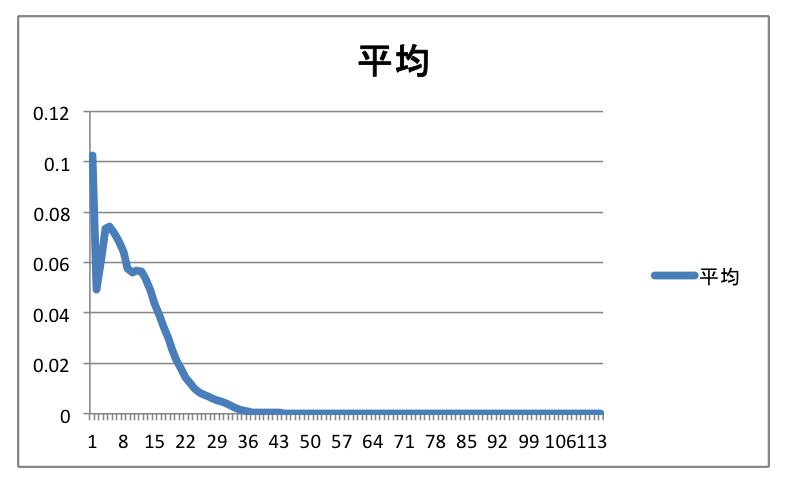
\includegraphics[width=10.0cm]{figs/2.eps}
  \caption{$B=E$_$r99?7$9$kMM;R!JJ?6QCM!K(B}
  \label{fig:level1-2}
 \end{center}
\end{figure}


\subsubsection{$B9M;!(B}
 $B>e5-$NFs$D$N?^$r8+$F(Bx$B<4$O<}B+2s?t$rI=$7!"(By$B<4$O8m:9$rI=$7$F$$$k!#?^#1$O(B10$B%Q%?!<%s$r$^$H$a<}B+2s?t$H8m:9$rI=$7$F$$$k!#?^#2$O(B10$B%Q%?!<%s$N%0%i%UJ?6Q$r$^$H$a$??^$G$"$k!#(B\\





\newpage

\section{Level2: 線形分離不可能なExOR問題への適用}
\subsection{課題説明}
階層型ニューラルネットワークをExOR問題へ適用し、
線形分離できない問題においても学習可能であることを確認する。
特にLevel2では、
この問題を解決するために中間層を導入することで拡張した階層型ニューラルネッ
トワークにより学習可能であることを確認する。



 %共通部分の結果及び考察
\subsection{階層型NNによる学習}
\subsubsection{最適なパラメータを探すためのアプローチ}
% 指定された条件下において学習が効率良く行われるパラメータの組み合わせを探
% すため、**して**することでパラメータを調整した。
% 
% (補足:全パターンを調べても良いし、いくつかのパターンを調べても良いが、
% どのような方法で調整したら良いかを考えよう)

$ETA,ALPHA,HIDDEN$を指定された範囲内でランダムな値に設定し,
プログラムを実行した.
パラメータの値の決定や,iteration数の平均値を求める処理は
次のシェルスクリプト(ソースコード\ref{level2})で行った.
ExOR問題は線形分離不可であるため,HIDDENの最小値を2としている.
最大値は特に指定されていないが,HIDDENを極端に大きくしすぎると
各パラメータの最適な組み合わせを見つけ出すのが困難になると考えたため,
最大値を16とした.


\lstinputlisting[caption=本levelで使用したシェルスクリプト,label=level2]{./level2figs/level2.sh}

このシェルスクリプトを数十回実行し,
iteration数の平均値が比較的小さい実行結果を10個分記録した.
その中で平均値が最小なものを選択し,グラフ化することにした.
また出力結果の文字列を処理するため,
bp\_mo\_exor.cの終了条件$FINISH$を出力するfprintf関数のstderrをstdoutへと変更を行った(ソースコード\ref{exor}).

\lstinputlisting[caption=bp\_mo\_exor.cの変更点,label=exor]{./level2figs/exor.c}


\subsubsection{実行結果}

% (補足:シード値10パターンで試した際の収束に要した学習回数と、その平均回数が分かるように明示してください。)

表\ref{table:level2}にシード値10パターンで試した際の収束に要した学習回数と,その最小の平均回数を示す.

\begin{table}[htb]
 \begin{center}
  \begin{tabular}[htb]{|r|l|} \hline
   シード値 & 収束した回数 \\ \hline \hline
   1000     & 37\\ \hline
   2000     & 45\\ \hline
   3000     & 52\\ \hline
   4000     & 44\\ \hline
   5000     & 50\\ \hline
   6000     & 53\\ \hline
   7000     & 39\\ \hline
   8000     & 29\\ \hline
   9000     & 38\\ \hline
   10000    & 39 \\ \hline \hline
   10試行の平均値 & 42 \\ \hline
  \end{tabular}
  \caption{階層型NNによるExOR問題の学習に要した回数}
  \label{table:level2}
 \end{center}
\end{table}

各パラメータが$ETA=1.26, ALPHA=0.94, HIDDEN=16$の時,表\ref{table:level2}のような結果が得られた.
その時の学習曲線は図\ref{fig:averageultimate}のようになる.
図\ref{fig:averageultimate}はseed値別にプロットしたグラフを元にsmooth uniqueオプションを用いて平均化を行い,得られたものである.

\begin{figure}[h]
 \begin{center}
  \includegraphics[width=10.0cm]{./level2figs/averageultimate.eps}
  \caption{重みを更新する様子(平均値)}
  \label{fig:averageultimate}
 \end{center}
\end{figure}


\subsubsection{考察}
ここでは,各パラメータとiteration数の関係について考察する. \\
 下記に平均iteration数が比較的小さい実行結果とそのときのパラメータの値を示す.
\begin{itembox}[c]{平均iteration数が小さい実行結果}
    {\small
        \verbatimtabinput{./level2figs/suitables.txt}
    }
\end{itembox}
10回の実行結果における共通点は,いずれも

\begin{itembox}[c]{平均iteration数が大きい実行結果}
    {\small
        \verbatimtabinput{./level2figs/unsuitables.txt}
    }
\end{itembox}


\newpage

\section{Level3: 応用事例:文字認識問題への適用}
\subsection{$B2]Bj@bL@(B}
$B3,AX7?(BNN$B$rJ8;zG'<1$KE,MQ$7!"9M;!$9$k!#(B
$BFC$K!"MQ0U$5$l$?65;U%G!<%?$HG'<1$N$7$d$9$5$K4X$9$k4X78@-$d!"(B
$B3X=,:GE,2=$N$?$a$N%Q%i%a!<%?$N%A%e!<%K%s%0$*$h$S!"(B
$B$h$j=@Fp@-$N9b$$G'<1J}K!$K4X$9$k8!F$$r9T$&!#(B

 %課題説明
\subsection{Level3.1: パラメータのチューニング}
\subsubsection{最適なパラメータを探すためのアプローチ}
指定された条件下において学習が効率良く行われるパラメータの組み合わせを探
すため、
hiddenを10から100まで10づつ増やしていき,etaを0.01から1.98まで0.01づつ増
やし,alphaを0.1から1.0まで0.1づつ増やしていきその中から一番値が小さい物
を探した.その動作をスクリプトを書いて実行させた.

\subsubsection{実行結果}
各パラメータが ET A = 1.26, ALPHA = 0.94, HIDDEN = 16 の時, 3 のよ
うな結果が得られた.その時の学習曲線 は図43 のようになる.
\begin{table}[htb]
 \begin{center}
  \caption{階層型NNによる文字認識問題の学習に要した回数}
  \label{table:level3}
  \begin{tabular}[htb]{r|l} \hline
   シード値 & 収束した回数 \\ \hline \hline
   1000 & 97 \\ \hline
   2000 & 81 \\ \hline
   3000 & 108 \\ \hline
   4000 & 106 \\ \hline
   5000 & 46 \\ \hline
   6000 & 130 \\ \hline
   7000 & 85 \\ \hline
   8000 & 89 \\ \hline
   9000 & 134 \\ \hline
   10000 & 84 \\ \hline \hline
   10試行の平均値 & 95.9 \\ \hline
  \end{tabular}
 \end{center}
\end{table}

\begin{figure}[h]
 \begin{center}
  \includegraphics[width=10.0cm]{ave.eps}
  \caption{重みを更新する様子(平均値)}
  \label{fig:level2}
 \end{center}
\end{figure}
\newpage



\subsection{Level3.2: $B%Q%i%a!<%?$H<}B+G=NO$N4XO"@-$K$D$$$F(B}
\subsubsection{$B4X78@-$r3NG'$9$k$?$a$N%"%W%m!<%A(B}
3$B$D$N%Q%i%a!<%?$,$I$N$h$&$J4X78$K$"$k$+$r8!>Z$9$k$?$a!"(B
$B%1!<%9(B1,2,,,$B$r@_Dj$7!"3X=,6J@~$+$i$=$N4X78@-$K$D$$$F9M;!$9$k!#(B

\subsubsection{$B7k2L(B}

\subsubsection{$B9M;!(B}


\subsection{Level3.3: $BG$0U$NI>2AMQ%G!<%?$rMQ$$$?I>2A(B}
\subsubsection{$B%"%W%m!<%A(B}
$B!J2>@b(B1$B!K(B\\
$B3X=,;~$N%G!<%?!J65;U%G!<%?!K$H$N0c$$$,>/$J$$DxG'<1N($,9b$/!"(B
$B5U$K65;U%G!<%?$H$N0c$$$,B?$$DxG'<1N($,Dc$/$J$k$H$N2>Dj$N2<!"(B
$BG!2?$K<($9I>2A%G!<%?$rMQ0U$7$?!#(B

$B!J2>@b(B2$B!K(B\\
$B3X=,;~$N%G!<%?!J65;U%G!<%?!K$H$N0c$$$,B?$$DxG'<1N($,9b$/!"(B
$B5U$K65;U%G!<%?$H$N0c$$$,>/$J$$DxG'<1N($,Dc$/$J$k$H$N2>Dj$N2<!"(B
$BG!2?$K<($9I>2A%G!<%?$rMQ0U$7$?!#(B

$B!JJdB-!'$=$l0J30$G$b9=$$$^$;$s$,!"(B
$B8!>Z$7$?$$FbMF$K1~$8$?2>@b$rN)$F!"(B
$B$=$N2>@b$r8!>Z$9$k$?$a$N%G!<%?$rMQ0U$7$^$7$g$&!K(B

\subsubsection{$B7k2L(B}

\subsubsection{$B9M;!(B}


\subsection{Level3.4: 認識率を高める工夫}
%下図のように入力されたデータが想定していた入力と比べてサイズが異なったり、
%位置がずれている等、数字の一部が欠けている以外にも多様な要因による
%データ(情報)の劣化が考えられる。
%認識率を高めるにはどのような点を工夫すれば良いか?
%どのような方法でも構わないので、検討せよ。
\subsubsection{対象とする問題点}
以下に対象とする問題点を列挙する.
\begin{itemize}
\item 与えられた数字のサイズが相対的に小さい
\item 与えられた数字のサイズが相対的に大きい
\item 与えられた数字の位置がずれている
\item 与えられた数字の周りにノイズが入っている
\end{itemize}

\subsubsection{改善方法の提案}
\begin{enumerate}
\item 数字のサイズが相対的に大きいもしくは小さいなどの場合は,
与えられた数字に対して拡大・縮小を行い,%与えられた数字を
学習用の数字に近づけた上で認識させる方法がある.
\item 数字の位置がずれている場合も同様に,
与えられた数字を中央に移動させたものを認識させる方法が考えられる.
\item 数字の周りにノイズが入っている場合は,
学習用の数字と与えられた数字とを重ね合わせてANDをとったものを
認識させる方法がある.
\end{enumerate}
% 平均化した後の値が大きい部分だけに注目すれば,
% ノイズが軽減された数字が浮かび上がり認識率が

\subsubsection{考察}
与えられた数字に対して拡大・縮小を行う方法の問題点として,
どの程度の拡大および縮小を行えばよいのかが不明な点である.
少しずつ拡大・縮小の度合いを大きくしていき,それを認識させる
ことを繰り返すという方法が考えられるが,
これはやや非効率なやり方である. \\
 数字を中央に移動させる方法は,
数字の縦横の比率から中央となる場所を割り出し,数字を移動させる
ため,比較的単純な処理となる. \\
%%  続いて,与えられた数字を中央に移動させる方法であるが,
%% これは与えられた数字の縦横の比率から中央を割り出し,そこ
%% 比較的簡単な作業となる. \\
% 重ね合わせて平均化する方法では,
 ANDをとる方法では,ANDをとることで与えられた数字と学習用の数字の
共通部分のみを抽出できるため,
%平均化した後に値が大きい部分だけに注目することで,
%数字の周りのノイズが軽減され,相対的に数字をくっきり
%認識できるようになるため,
認識率を格段に向上させることができる.
しかし,与えた数字と学習用の数字のどちらかが相対的に大きかったり,
互いの位置がずれていたりすると,この手法はあまり効果を発揮しない.
そのため,改善方法の提案で述べた1と2の方法と組み合わせることで,認識率を高めることができると考える.


\newpage
\section{levelX オプション課題}
\subsection{Level 3.1, 3.2 における複数シミュレーションを効率良く行い、集計
 するスクリプト作成やプログラム修正等。}
num.cを修正し実行すると,iterationの値だけが出力するようにした.以下のスク
リプトは./levelX/src/に置いてある
\begin{itemize}
 \item $fuga.perl$ \\
パラメータの値とseed値を変更しながらnn\_numを実行していく.結果は標準出力
       として出る.
 \item $hoge2.perl$ \\
fuga.perlで出た出力をファイルに保存しておきその中から一番収束するのが速
       い結果の行を出力する(sortコマンドのおかげで使用はしていない)
 \item $average.perl$ \\
学習曲線の平均値を出すプログラム.このプログラムを使用する際にはnum.cを修
       正してerrの値だけが出力されるようにし,その出力をseed値毎にファイ
       ルを分けて保存すると使用出来る.その際ファイルの名前
       は'rep[seed値].txt'にする.
\end{itemize}
\section{その他: 実験の内容・進め方に関するコメント等}
% (補足:
% 今後の為に参考にしたいので、情報工学実験2・探索アルゴリズム1,2で扱った
% 内容、実験の進め方等について意見があれば書いてください(当然、どのような
% 意見であってもレポートの評価を下げる事はしません。)。「授業評価アンケー
% ト」の際に書いてもらっても構いません。)


\vspace{+1.0cm}
% (補足:参考文献は thebibliography 環境を使って列挙し、
% 本文中で適切な箇所で引用するようにしましょう。
% 例えば下記文献は、アブストラクト中で引用しています)
\begin{thebibliography}{99}
\bibitem{info2-search2}
情報工学実験2: 探索アルゴリズムその2(當間)\\
\verb|http://www.eva.ie.u-ryukyu.ac.jp/~tnal/2011/info2/search2/|
\end{thebibliography}

\end{document}
